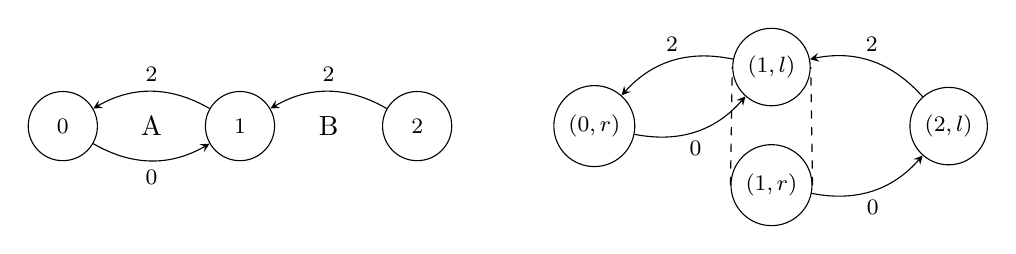
\begin{tikzpicture}[thin, scale=0.75]
  % Nodes
  \draw (-3,0) node(0) [circle,draw,minimum size=25] {\footnotesize \(0\)};
  \draw (0,0)  node(1) [circle,draw,minimum size=25] {\footnotesize \(1\)};
  \draw (3,0)  node(2) [circle,draw,minimum size=25] {\footnotesize \(2\)};

  % Edges
  \path[thin, ->, bend right, >=stealth] (1) edge[above] node {\footnotesize\(2\)} (0);
  \path[thin, ->, bend right, >=stealth] (2) edge[above] node {\footnotesize\(2\)} (1);
  \path[thin, ->, bend right, >=stealth] (0) edge[below] node {\footnotesize\(0\)} (1);
  % \path[thin, ->, bend right, >=stealth] (1) edge[below] node {\footnotesize\(0\)} (2);

  \draw (-1.5,0) node[] { A };
  \draw (1.5,0) node[] { B };

  \draw (6,0) node(B0) [circle,draw,minimum size=25] {\footnotesize \((0,r)\)};
  \draw (9,1.0)  node(B1l) [circle,draw,minimum size=25] {\footnotesize \((1,l)\)};
  \draw (9,-1.0)  node(B1r) [circle,draw,minimum size=25] {\footnotesize \((1,r)\)};
  \draw (12,0)  node(B2) [circle,draw,minimum size=25] {\footnotesize \((2,l)\)};

  \path[thin, ->, bend right, >=stealth] (B1l) edge[above] node {\footnotesize\(2\)} (B0);
  \path[thin, ->, bend right, >=stealth] (B2) edge[above] node {\footnotesize\(2\)} (B1l);
  \path[thin, ->, bend right, >=stealth] (B0) edge[below] node {\footnotesize\(0\)} (B1l);
  \path[thin, ->, bend right, >=stealth] (B1r) edge[below] node {\footnotesize\(0\)} (B2);

  \path[thin, dashed] (B1r.west) edge[below] node {} (B1l.west);
  \path[thin, dashed] (B1r.east) edge[below] node {} (B1l.east);


\end{tikzpicture}

%%% Local Variables:
%%% mode: latex
%%% TeX-master: "../paper"
%%% End:
